\lecture{Energy minimisation and the first finite element method}{Lecture 3 --- Thursday, August 27, 2026}{Math 6660 --- OneNote export \texttt{3rrd.pdf}, from p.~16}

\begin{roadmap}[Lecture 3]
\roadq{Where does ``minimum potential energy'' come from, and how does it turn
into a computer program?}
\begin{roadlist}
\item Define $F(w)=$ strain energy $-$ work done by the load. Minimising $F$
  over $\Vsp$ is \emph{exactly} the weak form --- proved, not asserted.
\item So the two derivations every FEM textbook gives, virtual work and energy
  minimisation, are one theorem stated twice.
\item Then the actual method: replace the infinite-dimensional $\Vsp$ by a
  finite-dimensional $\Vh$ of piecewise linear functions. That is
  \textbf{CG(1)}.
\item \textbf{Hat functions}: the basis in which each unknown coefficient
  \emph{is} a nodal displacement.
\end{roadlist}
\payoff{Seeing where the discretisation actually enters --- it is one step,
restricting the space, and nothing else about the problem changes.}
\end{roadmap}

% ==================================================================
\subsection*{Setup, restated}

\paragraph{2-pt BVP.}
\begin{equation}\label{eq:bvp3}
  -(au')' = f \ \text{ on } (0,1),
  \qquad u(0)=u(1)=0,
\end{equation}
with $f\in\Ck[(0,1)]{0}$, $a\in\Ck[(0,1)]{1}$, and
$0 < a_{1} \le a(x) \le a_{2} < \infty$ for all $x\in[0,1]$.

\paragraph{Variational problem.}
Find $u\in V$ such that
\begin{equation}\label{eq:var3}
  \int_{0}^{1} a\,u'v'\dx = \int_{0}^{1} f v\dx
  \qquad \forall\, v\in V,
\end{equation}
where
$V = \bigl\{ v : \int v^{2}\dx<\infty,\ \int (v')^{2}\dx<\infty,\ v(0)=v(1)=0 \bigr\}$.

\todoq{Page 16 writes the coefficient bound as $0\le a_{1} < a(x)\le a_{2}$,
but Lectures 1 and 2 both have $0 < a_{1}\le a(x)\le a_{2}$. The difference
matters: if $a_{1}=0$ were allowed, the $\eps^{2}$ coefficient in Claim
\textcircled{\scriptsize2} below could vanish and the minimiser would stop
being unique. I have used the Lecture 1 version.}

% ==================================================================
\subsection*{The ``energy'' minimisation problem}

Define the following energy functional:
\begin{equation}\label{eq:Fdef}
  F(w) \;=\;
  \underbrace{\frac12\int_{0}^{1} a\,(w')^{2}\dx}_{\text{internal energy}}
  \;-\;
  \underbrace{\int_{0}^{1} f\,w\dx}_{\text{potential energy}}
  \qquad w \text{ is a function.}
\end{equation}

\begin{mechanics}[$F$ is the total potential energy $\Pi$]
This is the most familiar object in the course so far, under a name you have
used since undergraduate structures. With $a=EA$ and $w'=\eps$:
\[
  F(w) \;=\;
  \underbrace{\tfrac12\int_{0}^{1} EA\,\eps^{2}\dx}_{\text{strain energy } U}
  \;-\;
  \underbrace{\int_{0}^{1} f\,w\dx}_{\substack{\text{work done by the applied}\\\text{load through } w}}
  \;=\; U - W \;=\; \Pi .
\]
So the Min Problem below is the \textbf{principle of minimum total potential
energy}: of all kinematically admissible displacement fields, the one that
actually occurs is the one that minimises $\Pi$. That is the principle behind
Rayleigh--Ritz, and --- as this lecture proves --- behind FEM.

Your own margin note ``not total energy'' is exactly right and worth keeping:
$F$ is the total \emph{potential} energy. There is no kinetic term because the
problem is static.
\end{mechanics}

\begin{pitfall}[``kinetic energy $-$ potential energy'' is the wrong label]
My notes annotate \eqref{eq:Fdef} with ``kinetic energy $-$ potential energy''.
That label belongs to a different principle and should not be attached here.

$L = T - V$ (kinetic minus potential) is the \emph{Lagrangian}, and the
principle that makes it stationary is Hamilton's principle, which governs
\emph{dynamics}. Equation \eqref{eq:Fdef} is static: the first term is
$\tfrac12\int EA\eps^{2}$, which is \textbf{strain energy}, not kinetic energy
--- there is no velocity anywhere in this problem.

The reason the analogy gets drawn is structural, and it is worth seeing
clearly: both functionals are ``a positive quadratic term minus a linear
term,'' and in both cases the physical state makes the functional stationary.
That shared shape is real. But the physical content of the quadratic term is
different, and conflating them will cause trouble later when the course reaches
time-dependent problems, where a genuine kinetic term $\tfrac12\int\rho\dot u^2$
appears \emph{alongside} the strain energy.
\end{pitfall}

\paragraph{Min problem.} Find $u\in V$ such that
\begin{equation}\label{eq:min}
  F(u) \le F(w) \qquad \forall\, w\in V .
\end{equation}

% ==================================================================
\subsection*{Claim: the Min Problem and the variational problem are equivalent}

\begin{theorem}\label{thm:equiv}
The minimisation problem \eqref{eq:min} and the variational problem
\eqref{eq:var3} are equivalent.
\end{theorem}

% ---------- direction 1 ----------
\paragraph{\textcircled{\scriptsize1} (variational problem) $\Rightarrow$ (Min Prob).}

Assume $u\in V$ satisfies $\int_{0}^{1}au'v'\dx = \int_{0}^{1}fv\dx$ for all
$v\in V$. Let $w\in V$, and set $w = u+v$. Then
\begin{align}
  F(w) &= F(u+v) \notag\\[2pt]
   &= \frac12\int_{0}^{1} a\,(u'+v')^{2}\dx
      - \int_{0}^{1} f u\dx - \int_{0}^{1} f v\dx \notag\\[2pt]
   &= \frac12\int_{0}^{1} a(u')^{2}\dx
    + \underbrace{\int_{0}^{1} a u'v'\dx}_{\text{(A)}}
    + \frac12\int_{0}^{1} a(v')^{2}\dx
    - \int_{0}^{1} f u\dx
    - \underbrace{\int_{0}^{1} f v\dx}_{\text{(B)}} .
    \label{eq:expand}
\end{align}
Terms (A) and (B) cancel, since (A)$\,-\,$(B)$\,=0$ is exactly the variational
problem. What remains is
\begin{equation}\label{eq:completed}
  \boxed{\;F(w) = F(u) + \frac12\int_{0}^{1} a\,(v')^{2}\dx\;}
\end{equation}
and since $a\ge a_{1}>0$, the last term is $\ge 0$. Therefore
\begin{equation}
  F(w) \;\ge\; F(u) \qquad \forall\, w\in V .
\end{equation}

\begin{intuition}[deviating from equilibrium always costs energy]
Equation \eqref{eq:completed} is the whole content of the minimum potential
energy principle, and it is worth reading slowly.

Take the true equilibrium shape $u$ and perturb it by \emph{any} admissible
amount $v$. The potential energy does not change by an amount proportional to
$v$ --- that first-order term is exactly (A)$-$(B), and it vanishes
\emph{because $u$ is in equilibrium}. What is left is a purely second-order
term, $\tfrac12\int a(v')^{2}$, which is the strain energy stored by the
perturbation itself, and it is always positive.

So: \textbf{the equilibrium configuration sits at the bottom of an energy
well.} Any wrong shape you propose stores extra strain energy and has higher
potential energy, by precisely the strain energy of your error. This is also
the algebraic ancestor of Céa's lemma and of ``FEM is too stiff'': when the
course later restricts to $\Vh$, the best you can do is the shape in $\Vh$ that
gets furthest down this well, and it can never get lower than $u$ itself.
\end{intuition}

\begin{recall}[this is just completing the square]
In finite dimensions with $\Kmat$ symmetric positive definite,
$F(\bm{w})=\tfrac12\bm{w}^{T}\Kmat\bm{w}-\bm{w}^{T}\Fvec$. Putting
$\bm{w}=\bm{u}+\bm{v}$ with $\Kmat\bm{u}=\Fvec$ gives
\[
  F(\bm{u}+\bm{v}) = F(\bm{u}) + \bm{v}^{T}(\Kmat\bm{u}-\Fvec)
                     + \tfrac12\bm{v}^{T}\Kmat\bm{v}
                   = F(\bm{u}) + \tfrac12\bm{v}^{T}\Kmat\bm{v},
\]
which is \eqref{eq:completed} term for term. Solving $\Kmat\bm{u}=\Fvec$ and
minimising $F$ are the same task --- exactly what Theorem~\ref{thm:equiv} says
in the continuous setting.
\end{recall}

\todoq{My notes conclude ``$F(w) > F(u)$'' with a strict inequality, but
\eqref{eq:completed} gives equality when $v=0$ (\ie $w=u$). It should be
$F(w)\ge F(u)$, with equality iff $w=u$. Strictness holds only for $w\ne u$.}

% ---------- direction 2 ----------
\paragraph{\textcircled{\scriptsize2} (Min Prob) $\Rightarrow$ (variational problem).}

Assume $u\in V$ satisfies $F(u)\le F(w)$ for all $w\in V$. Let
\begin{equation}
  g(\eps) = F(u+\eps v),
  \qquad\text{where } v\in V \text{ is arbitrary but fixed.}
\end{equation}
Expanding,
\begin{align}
  g(\eps) &= \frac12\int_{0}^{1} a\,(u'+\eps v')^{2}\dx
             - \int_{0}^{1} f\,(u+\eps v)\dx \notag\\[2pt]
    &= \frac12\int_{0}^{1} a(u')^{2}\dx
     + \eps\int_{0}^{1} a u'v'\dx
     + \frac12\eps^{2}\!\int_{0}^{1} a(v')^{2}\dx
     - \int_{0}^{1} f u\dx
     - \eps\int_{0}^{1} f v\dx .
\end{align}

\noindent
$g(\eps)$ is a quadratic polynomial in $\eps$ with a positive quadratic term.
The unique global minimiser happens at $\eps=0$, so $g'(0)=0$. Since
\begin{equation}\label{eq:gprime}
  g'(\eps) = \int_{0}^{1} a\,u'v'\dx - \int_{0}^{1} f v\dx
             + \eps\int_{0}^{1} a\,(v')^{2}\dx,
\end{equation}
setting $\eps=0$ gives
\begin{equation}
  g'(0) = \int_{0}^{1} a\,u'v'\dx - \int_{0}^{1} f v\dx = 0,
\end{equation}
which is exactly the variational problem. Since $v$ was arbitrary, the
variational problem is completely equivalent to this energy minimisation.
\qed

\todoq{Page 19 writes $g'(\eps)=\int u'v'\dx - \int fv\dx$, dropping the
coefficient $a$ from the first term, and the $+$ before the $\eps$ term is
missing. Both are present on the following page, so I have restored them in
\eqref{eq:gprime}.}

\begin{intuition}[$g'(0)=0$ is $\delta\Pi = 0$]
This direction is the \emph{first variation}, written out longhand. When a
mechanics text writes $\delta\Pi=0$, the operation it means is precisely
\[
  \delta\Pi = \frac{\dd}{\dd\eps}\,\Pi(u+\eps\,\delta u)\bigg|_{\eps=0} = 0 .
\]
The trick of introducing a scalar $\eps$, differentiating an ordinary
one-variable function, and setting $\eps=0$ is how a ``variation'' is made
rigorous: it converts a question about a functional on an
infinite-dimensional space into single-variable calculus along one line
through $u$.

$v$ is again the virtual displacement, and ``$v$ arbitrary but fixed'' is
``for an arbitrary admissible virtual displacement.'' So this direction says:
\emph{minimum potential energy $\Rightarrow$ virtual work}. Direction
\textcircled{\scriptsize1} said the converse. Together, they are the statement
that the energy principle and the virtual-work principle are two descriptions
of one fact.
\end{intuition}

\begin{pitfall}[the positive $\eps^{2}$ coefficient is doing real work]
Note the exact phrase: ``a quadratic polynomial in $\eps$ \emph{with a positive
quadratic term}.'' That coefficient is $\tfrac12\int a(v')^{2}$, and it is
positive only because $a\ge a_{1}>0$. It is the same coercivity assumption
that gave uniqueness in Lecture 2.

Why it matters: $g'(0)=0$ alone only makes $u$ a \emph{stationary} point.
A parabola opening upward makes it a minimum; if the quadratic coefficient
could be zero or negative, $g'(0)=0$ would still hold at a saddle or a maximum,
and \eqref{eq:min} would be false.

You have met the moment this fails. In buckling, the second variation of the
potential energy loses positive-definiteness at the critical load --- the
equilibrium is still stationary, but it stops being a minimum, and the
structure snaps to a different configuration. Everything in this course
assumes we are safely on the positive-definite side of that.
\end{pitfall}

\begin{dictionary}[the three formulations]
strong form $-(au')'=f$ & pointwise equilibrium of a differential slice \\
variational problem $\int au'v' = \int fv\ \forall v$ & principle of virtual work, $\delta W_{\text{int}}=\delta W_{\text{ext}}$ \\
min problem $F(u)\le F(w)$ & principle of minimum total potential energy \\
$g'(0)=0$ & $\delta\Pi=0$, stationary potential energy \\
$\eps^{2}$ coefficient $>0$ & $\delta^{2}\Pi>0$: the equilibrium is stable \\
\end{dictionary}

\begin{intuition}[why this equivalence is worth a whole lecture]
Three problems are now known to be the same object: the BVP (Lecture 2), the
variational problem, and the minimisation problem. That is not bookkeeping ---
each gives a different way to \emph{build} a numerical method:
\begin{itemize}[leftmargin=1.4em,itemsep=2pt]
  \item From the variational form, restrict $v$ to $\Vh$ $\Rightarrow$
        \textbf{Galerkin}.
  \item From the energy form, minimise $F$ over $\Vh$ $\Rightarrow$
        \textbf{Rayleigh--Ritz}.
\end{itemize}
For this problem --- symmetric $a$, positive definite --- the two produce the
\emph{identical} linear system. That is why the mechanics literature calls FEM
``Rayleigh--Ritz'' and the mathematics literature calls it ``Galerkin,'' and
why both are right.

The equivalence breaks when the operator is not symmetric: an advection term
$b u'$ has no energy functional to minimise, so Rayleigh--Ritz has nothing to
work with, while Galerkin still applies. That is the first hint of why the
course will keep proving things about $a(\cdot,\cdot)$ rather than about $F$.
\end{intuition}

% ==================================================================
\subsection*{Our first finite element method}

\textbf{Idea:} solve the variational problem (or the Min problem) approximately
by replacing $V$ with a finite-dimensional subspace $\Vh$.

Let $\Th$ be a mesh on $(0,1)$:
\begin{center}
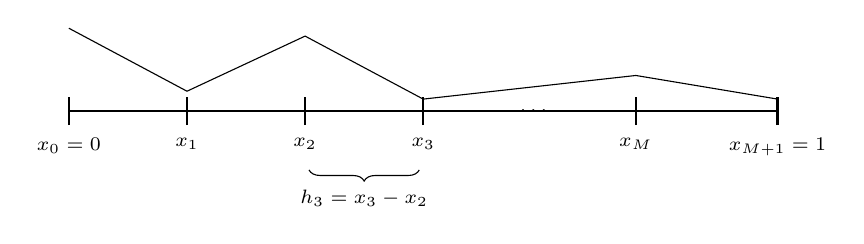
\begin{tikzpicture}[scale=1.0]
  \draw[thick] (0,0) -- (9,0);
  \foreach \x/\lab in {0/{x_{0}=0}, 1.5/{x_{1}}, 3/{x_{2}}, 4.5/{x_{3}}, 7.2/{x_{M}}, 9/{x_{M+1}=1}}{
    \draw[thick] (\x,-0.18) -- (\x,0.18);
    \node[below] at (\x,-0.22) {\scriptsize$\lab$};
  }
  \node at (5.9,0.0) {\scriptsize$\cdots$};
  % a piecewise linear function on the mesh
  \draw[thin] (0,1.05) -- (1.5,0.25) -- (3,0.95) -- (4.5,0.15) -- (7.2,0.45) -- (9,0.15);
  % brace for h_j
  \draw[decorate,decoration={brace,amplitude=4pt,mirror},thin]
        (3.05,-0.75) -- (4.45,-0.75);
  \node[below] at (3.75,-0.88) {\scriptsize$h_{3}=x_{3}-x_{2}$};
\end{tikzpicture}
\end{center}
Let
\begin{equation}
  h_{j} = x_{j} - x_{j-1},
  \qquad j = 1,2,\dots,M+1 .
\end{equation}

\medskip
The simplest $\Vh\subset V$ is the \textbf{space of continuous piecewise linear
polynomials on $\Th$}. This is called the
\begin{equation}
  \boxed{\textbf{CG(1) method}}
  \qquad
  \underbrace{\text{Continuous Galerkin method}}_{}
  \text{ with polynomials of degree } 1 .
\end{equation}

\begin{mechanics}[CG(1) is the 2-node bar element]
Strip the name and this is the element you have built by hand. ``Continuous
piecewise linear on $\Th$'' means: straight-line displacement within each
element, matching at the nodes. That is the linear 2-node bar --- constant
strain per element, and in 2D its cousin is the constant-strain triangle.

Two words carry weight:
\begin{itemize}[leftmargin=1.4em,itemsep=2pt]
  \item \textbf{Continuous}: the pieces join at the nodes. This is what makes
        $\Vh\subset V$ (``conforming''), and Lecture 2 explained why --- a jump
        would mean infinite strain energy, so a discontinuous $\Vh$ would not
        be a subspace of $V$ at all. It is your $C^{0}$ compatibility
        requirement.
  \item \textbf{(1)}: polynomial degree. CG(2) is the 3-node quadratic bar,
        and so on. Raising it is $p$-refinement; shrinking $h_{j}$ is
        $h$-refinement.
\end{itemize}
Note also that the mesh spacing $h_j$ is allowed to vary --- the elements need
not be equal length. That is local mesh refinement, available from the very
first definition.
\end{mechanics}

\medskip
Any function in $\Vh$ can be uniquely written as
\begin{equation}\label{eq:expansion}
  U(x) = \sum_{j=1}^{M} \xi_{j}\,\phih_{j}(x),
\end{equation}
where the $\xi_{j}$ are coefficients and $\phih_{j}(x)$ is the hat function
associated with $x_{j}$:
\begin{equation}\label{eq:hat}
  \phih_{j}(x) = \begin{cases}
    \dfrac{x-x_{j-1}}{h_{j}}, & x_{j-1}\le x\le x_{j},\\[10pt]
    \dfrac{x_{j+1}-x}{h_{j+1}}, & x_{j}\le x\le x_{j+1},\\[8pt]
    0, & \text{everything else, outside those limits.}
  \end{cases}
\end{equation}

\begin{center}
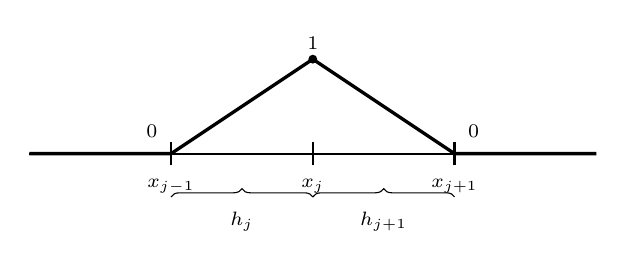
\begin{tikzpicture}[scale=1.0]
  \draw[thick] (-0.6,0) -- (6.6,0);
  \draw[very thick] (-0.6,0) -- (1.2,0) -- (3,1.2) -- (4.8,0) -- (6.6,0);
  \foreach \x/\lab in {1.2/{x_{j-1}}, 3/{x_{j}}, 4.8/{x_{j+1}}}{
    \draw[thick] (\x,-0.15) -- (\x,0.15);
    \node[below] at (\x,-0.2) {\scriptsize$\lab$};
  }
  \fill (3,1.2) circle (1.6pt);
  \node[above] at (3,1.2) {\scriptsize$1$};
  \node[left]  at (1.15,0.28) {\scriptsize$0$};
  \node[right] at (4.85,0.28) {\scriptsize$0$};
  \draw[decorate,decoration={brace,amplitude=3pt},thin] (1.2,-0.55) -- (3,-0.55);
  \node[below] at (2.1,-0.62) {\scriptsize$h_{j}$};
  \draw[decorate,decoration={brace,amplitude=3pt},thin] (3,-0.55) -- (4.8,-0.55);
  \node[below] at (3.9,-0.62) {\scriptsize$h_{j+1}$};
\end{tikzpicture}
\end{center}

\begin{intuition}[the coefficients \emph{are} the nodal displacements]
The definition \eqref{eq:hat} is engineered so that
\[
  \phih_{j}(x_{i}) = \delta_{ij}
  \qquad\text{(one at its own node, zero at every other node),}
\]
and therefore, evaluating \eqref{eq:expansion} at $x_{i}$,
\[
  U(x_{i}) = \sum_{j} \xi_{j}\,\phih_{j}(x_{i}) = \xi_{i}.
\]
So $\xi_{j}$ is not an abstract expansion coefficient --- it is
\textbf{the displacement of node $j$}. This is the property that makes FEM
usable: the unknowns you solve for are physically meaningful, boundary
conditions are imposed by setting nodal values directly, and the answer can be
plotted without post-processing. A basis without this property (a Fourier
basis, say) gives coefficients that mean nothing individually.

This is called a \emph{nodal} or \emph{Lagrange} basis, and $\xi$ is your
DOF vector $\Uvec$.
\end{intuition}

\begin{pitfall}[why the sum starts at $j=1$ and stops at $M$]
The mesh has nodes $x_{0},\dots,x_{M+1}$ --- that is $M+2$ nodes and $M+1$
elements. But \eqref{eq:expansion} sums only $j=1,\dots,M$: the
\emph{interior} nodes. The hats $\phih_{0}$ and $\phih_{M+1}$ at the two
endpoints are deliberately left out.

That omission \emph{is} the boundary condition. Every function built from
interior hats automatically satisfies $U(0)=U(1)=0$, so $\Vh\subset V$ by
construction rather than by an extra constraint. In solver terms, this is
eliminating the fixed DOFs from the system instead of penalising them, and it
is why $\dim\Vh = M$ and the stiffness matrix will be $M\times M$.

If the problem had $u(0)=g\ne0$ you would put $\phih_{0}$ back with its
coefficient \emph{fixed} at $g$ and move its column to the right-hand side ---
which is the discrete version of the trial/test distinction flagged in
Lecture 2.
\end{pitfall}

\begin{intuition}[what happens next, and why the mesh makes $\Kmat$ sparse]
The lecture stops at the definition of $\Vh$, but the next step is mechanical.
Substituting $U=\sum_{j}\xi_{j}\phih_{j}$ into \eqref{eq:var3} and testing
against each $\phih_{i}$ turns the variational problem into
\[
  \Kmat\bm{\xi}=\Fvec,
  \qquad
  K_{ij} = \int_{0}^{1} a\,\phih_{j}'\,\phih_{i}'\dx,
  \qquad
  F_{i} = \int_{0}^{1} f\,\phih_{i}\dx .
\]
Two features fall straight out of \eqref{eq:hat}:
\begin{itemize}[leftmargin=1.4em,itemsep=2pt]
  \item $\phih_{j}$ is nonzero only on $[x_{j-1},x_{j+1}]$, so
        $K_{ij}=0$ unless $\abs{i-j}\le1$: the stiffness matrix is
        \textbf{tridiagonal}. Sparsity is a consequence of choosing basis
        functions with small support, nothing more.
  \item $\phih_{j}'$ is \emph{constant} on each element ($\pm1/h$), so the
        element integrals can be done exactly by hand --- which is why the
        classical bar-element stiffness $\frac{EA}{h}\begin{psmallmatrix}1&-1\\-1&1\end{psmallmatrix}$
        looks the way it does.
\end{itemize}
\end{intuition}
